\section{Introduction}

It has been a hot research direction of parallelism in the recent two or 
three decades. A bunch of frameworks are invented to help programmers 
write better parallelized, more reliable and clearer codes. OpenMP, MPI, 
POSIX thread libraries, and big vendors like MapReduce, Amazon EC2 have made
it extremely easy and common to write a parallel program. 

There has always been, however, a gap between research work and practical 
multithreaded programs. Silas pointed out in 2010 that a great number of 
multithreaded programs will reach parallelization bottleneck when the 
number of cores scale up. For example, \emph{memcached}, a popular in 
memory cache program, scales poorly (as showed in figure 
\ref{figure:memcached})
by the number of cores on Linux 
operating system, even if the codes is very carefully written. The main 
reason of this bottleneck is a piece of kernel codes leads to significant 
overhead in kernel time, which limits the parallelism of \emph{memcached}.
\begin{figure}[H]
\center
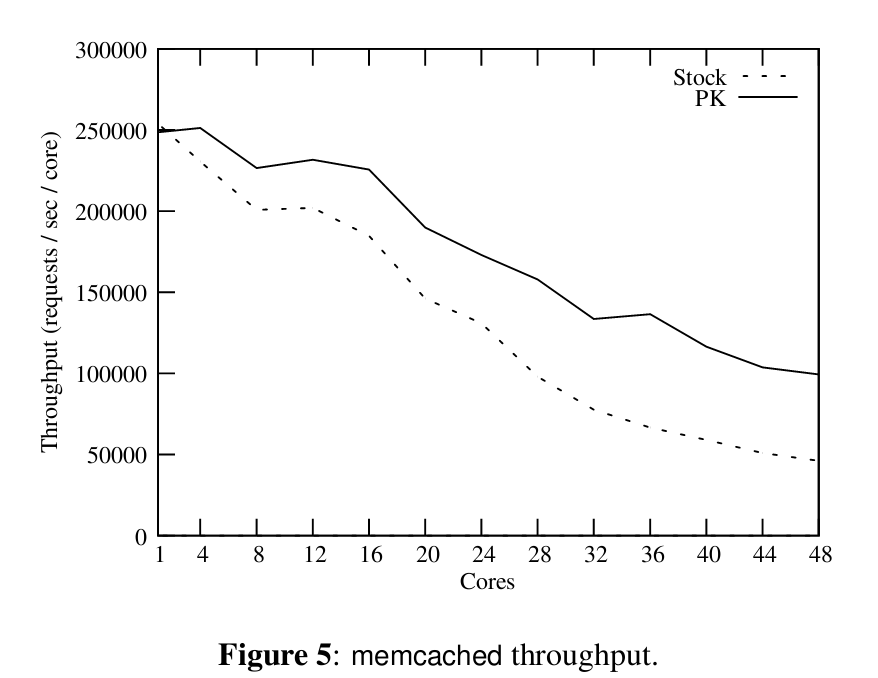
\includegraphics[width=0.8\linewidth]{figures/memcachced_scal.png}
\caption{Parallelism bottleneck of \emph{memcached} on Linux} 
\label{figure:memcached}
\end{figure}
Operating system kernel is one external factor that might limit the 
parallelism of our programs, but definitely not the only one. I/O speed, 
network condition, hardware configuration, scheduling algorithm and many
more might change the scalability curve or multithreaded programs. 

In this project, we target the influence of virtual machines/emulators on 
the parallelism of multithreaded programs. Here're some reasons why we choose
VM/emulator for study.
\begin{itemize}
\item It has been a short time from VMs/emulators start to support multicore
systems. Developers and researchers might not be able to do careful study 
on parallelism support of general mulithreaded programs.
\item VMs/emulators have to somehow control the schedule of CPU slices 
without careful consideration of what's running on the guest machine. 
\item Many VMs/emulators are open-source.
\end{itemize}

We selected QEMU as emulator to run some popular multithreaded benchmarks
(splash2, REDIS), as well as some dedicated microbenchmarks to evalute 
specific parallelization properties. Here're briefly our results. 

\begin{enumerate}
\item QEMU causes significantly runtime slowdown (approximately 20 times) of all
the benchmarks.
\item QEMU limits the parallelism of some CPU-intensive benchmarks (FFT)
\item QEMU does not have notable scalability issue for any particular kind of 
synchronization operations. 
\end{enumerate}

\paragraph{Roadmap} First, we will show some related works in section 
\ref{sec:rel}. In section \ref{sec:setup}, we will describe the setup of 
our evaluation system and benchmarks. Then in section \ref{sec:res}, we will 
show the result obtained in the experiments. With the results, we wrote some 
dedicated micro-benchmarks and evaluted scalability of synchronizaion operations
in section \ref{sec:mic}.
